\documentclass{article}
\usepackage[utf8]{inputenc}

\title{KREPE Control Board}
\author{Matt Ruffner}
\date{March 2020}

\usepackage{url}
\usepackage{float}
\usepackage{natbib}
\usepackage{graphicx}
\usepackage{listings}
\usepackage{fullpage}
\usepackage{hyperref}
\hypersetup{
    colorlinks=true,
    linkcolor=blue,
    filecolor=magenta,      
    urlcolor=cyan,
}

\begin{document}

\maketitle
\tableofcontents
\newpage
\listoffigures
\listoftables
\newpage

\section{Introduction}

This document has pin names and connections, along with implementation notes and design choice explanations. Schematic designs for this board were adapted from previous designs of KRUPS projects here at the University of Kentucky. Battery charging, improved activation circuitry, a newer IMU, and wireless debug capability are the main additions to previous designs. Newer thermocouple conversion ICs were also added to replace the EOL product that was in previous designs. Activation subsytems and criteria are also outlined.

The following sections outline the electrical connections for control of the board w.r.t. the Teensy 3.5 microcontroller, as well as several relevant subsystem specifications and links to datasheets. Charging and switch wiring for activation are also explained. Schematics are in Appendix \ref{appa}, along with Teensy 3.5 reference card images.

\subsection{Primary Activation}
Primary activation is triggered by a pin pull out the KREPE enclosure performed by astronauts. Once the pin is pulled, the flight computer is powered on and in standy mode, consuming a minimal amount of power. No radios are powered on in standy mode to ensure no interference with ISS activities. 

The \texttt{POWER\_SW} header must closed for protected battery or USB voltage to be applied to the Teensy's VIN pin, powering on the system. The location of these connection points can be seen in Fig. \ref{fig:board-top} labelled on the silk screen in the left middle of the PCB. A rendering of the bottom of the board is shown in Fig. \ref{fig:board-bottom}.

An end-to-end schematic showing battery protection and device activation is shown in Fig. \ref{fig:activation-circuitry}.

\begin{figure}[H]
    \centering
    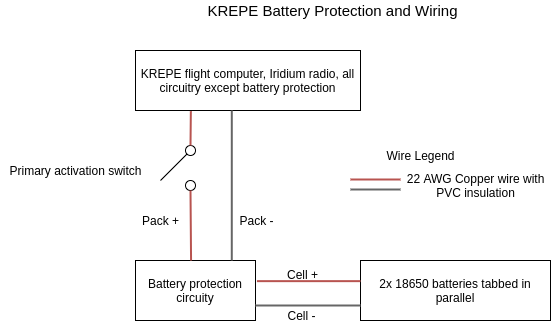
\includegraphics[width=0.6\textwidth]{images/krepe-electrical-overview.png}
    \caption{Activation and battery protection schematic overview.}
    \label{fig:activation-circuitry}
\end{figure}


\begin{figure}[H]
    \centering
    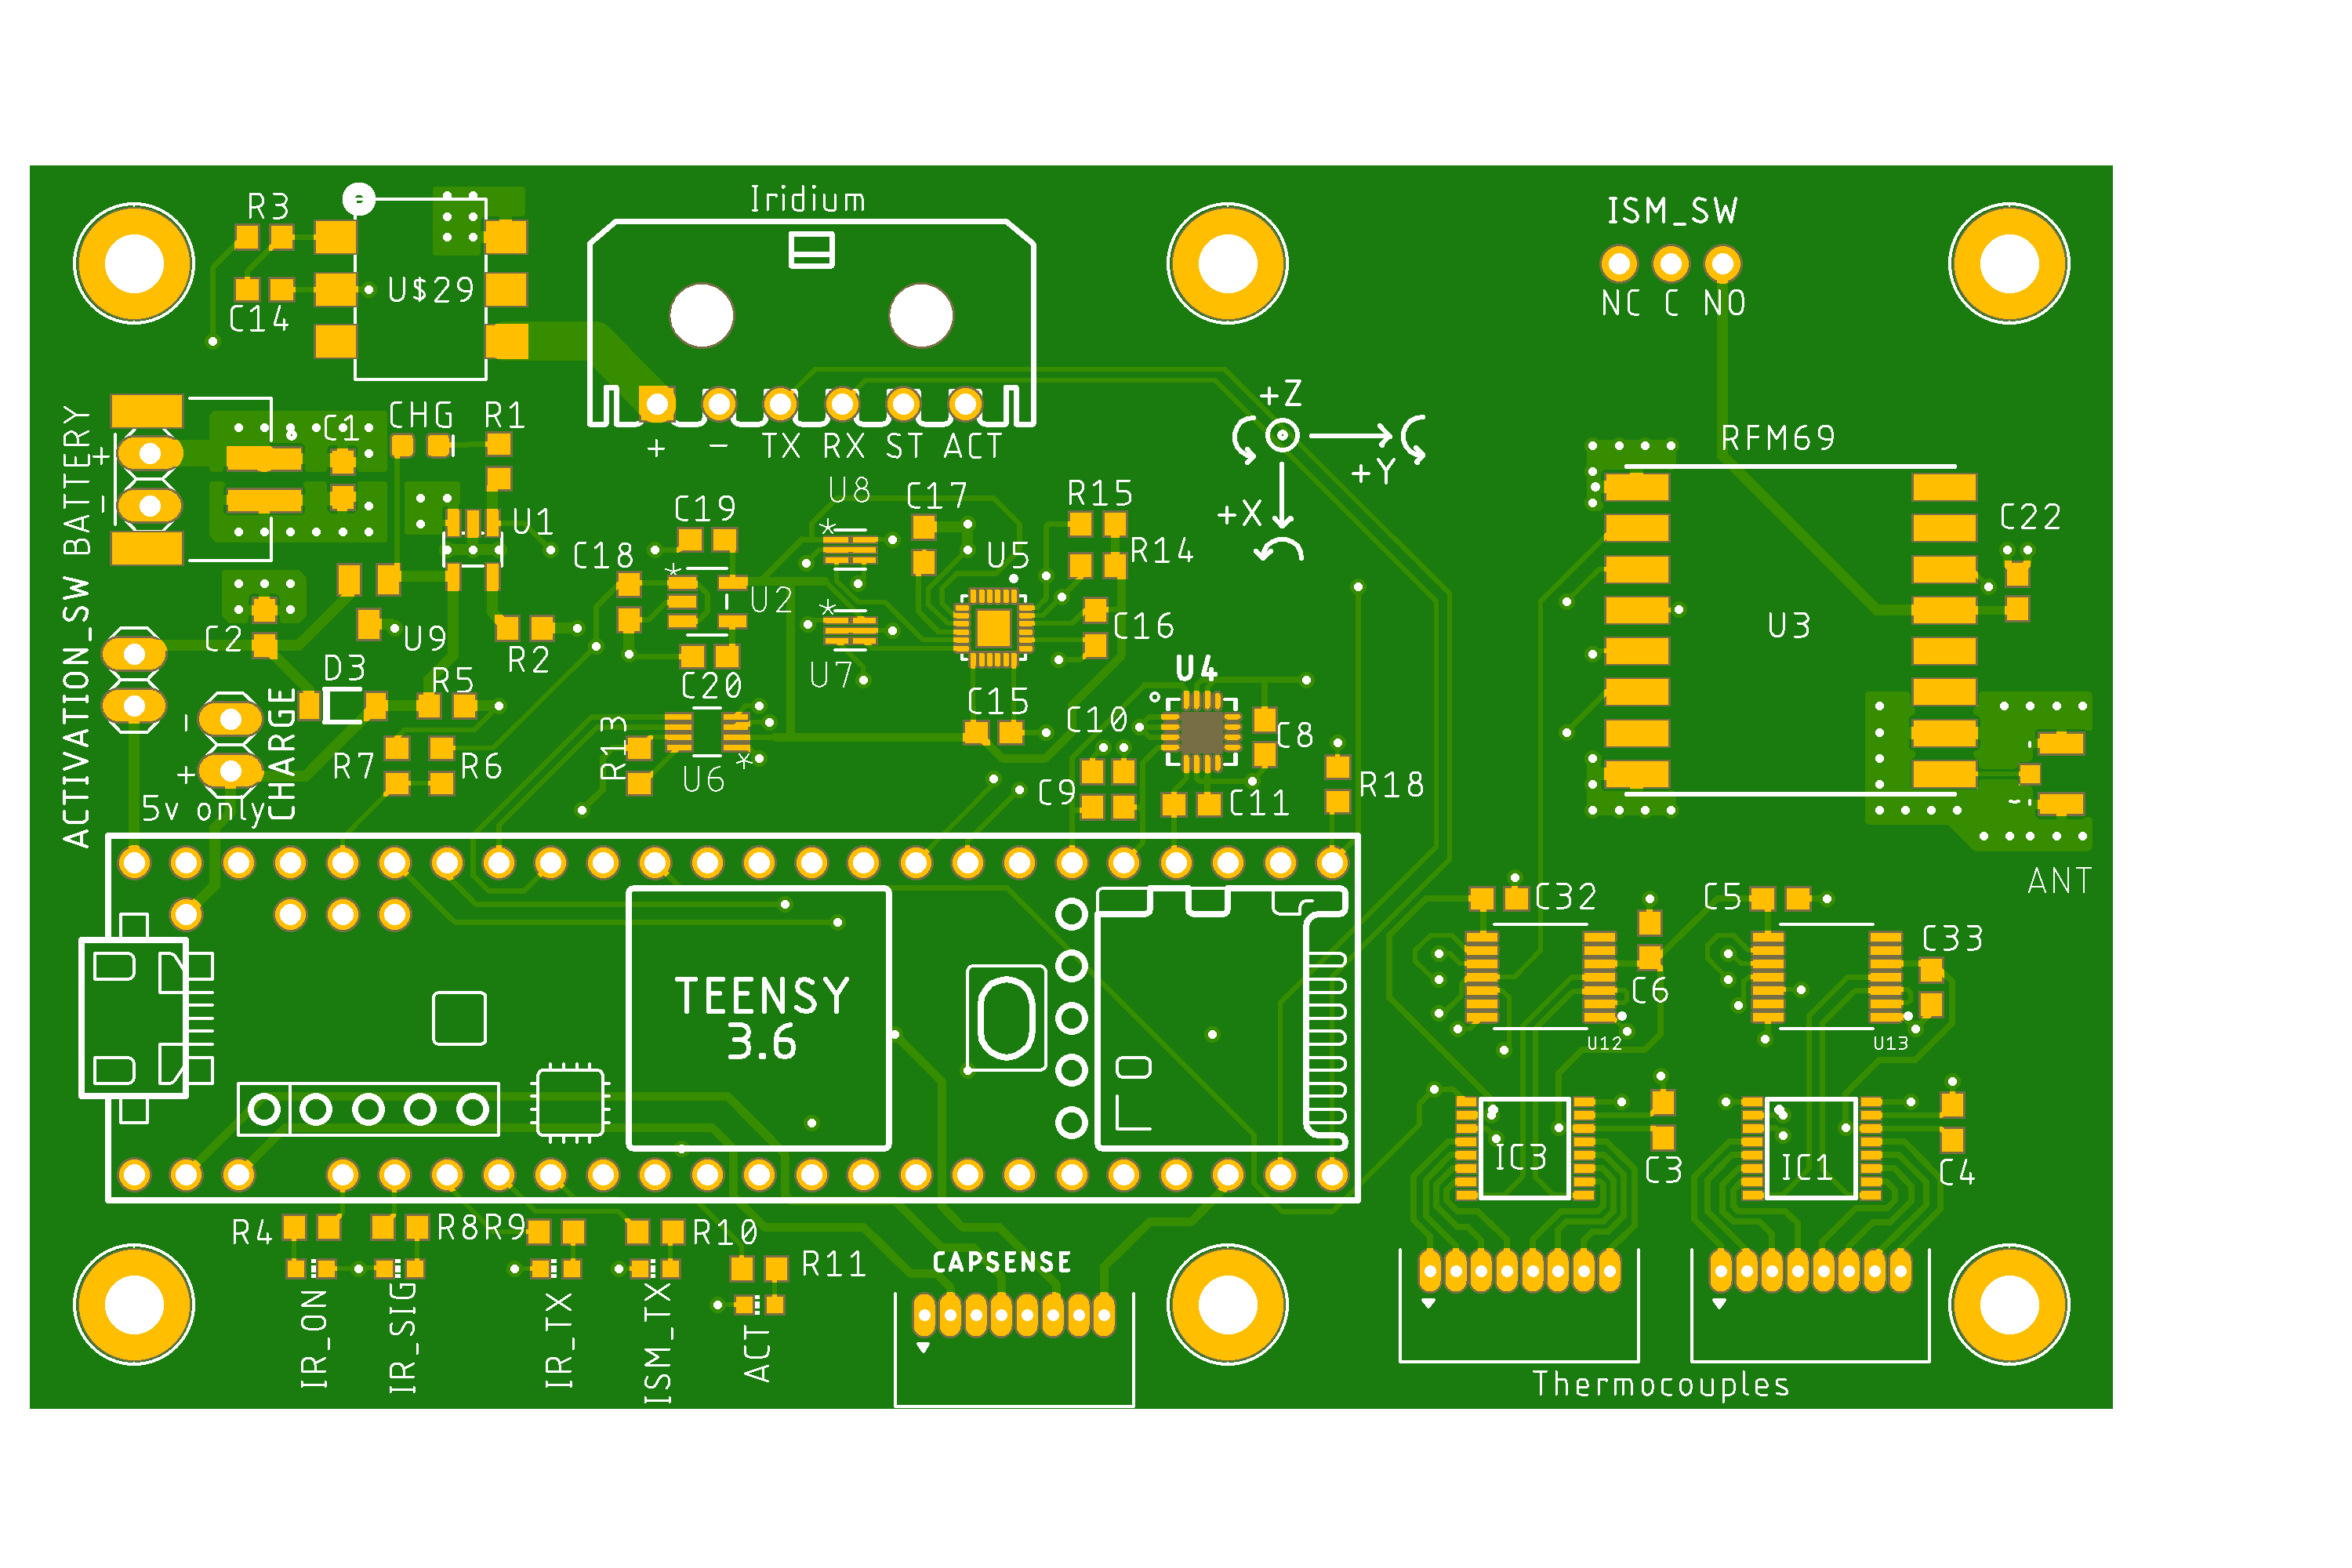
\includegraphics[width=\textwidth]{images/krepe-top.png}
    \caption{Rendering of the top of the KREPE control board, V1.1.}
    \label{fig:board-top}
\end{figure}


\begin{figure}[H]
    \centering
    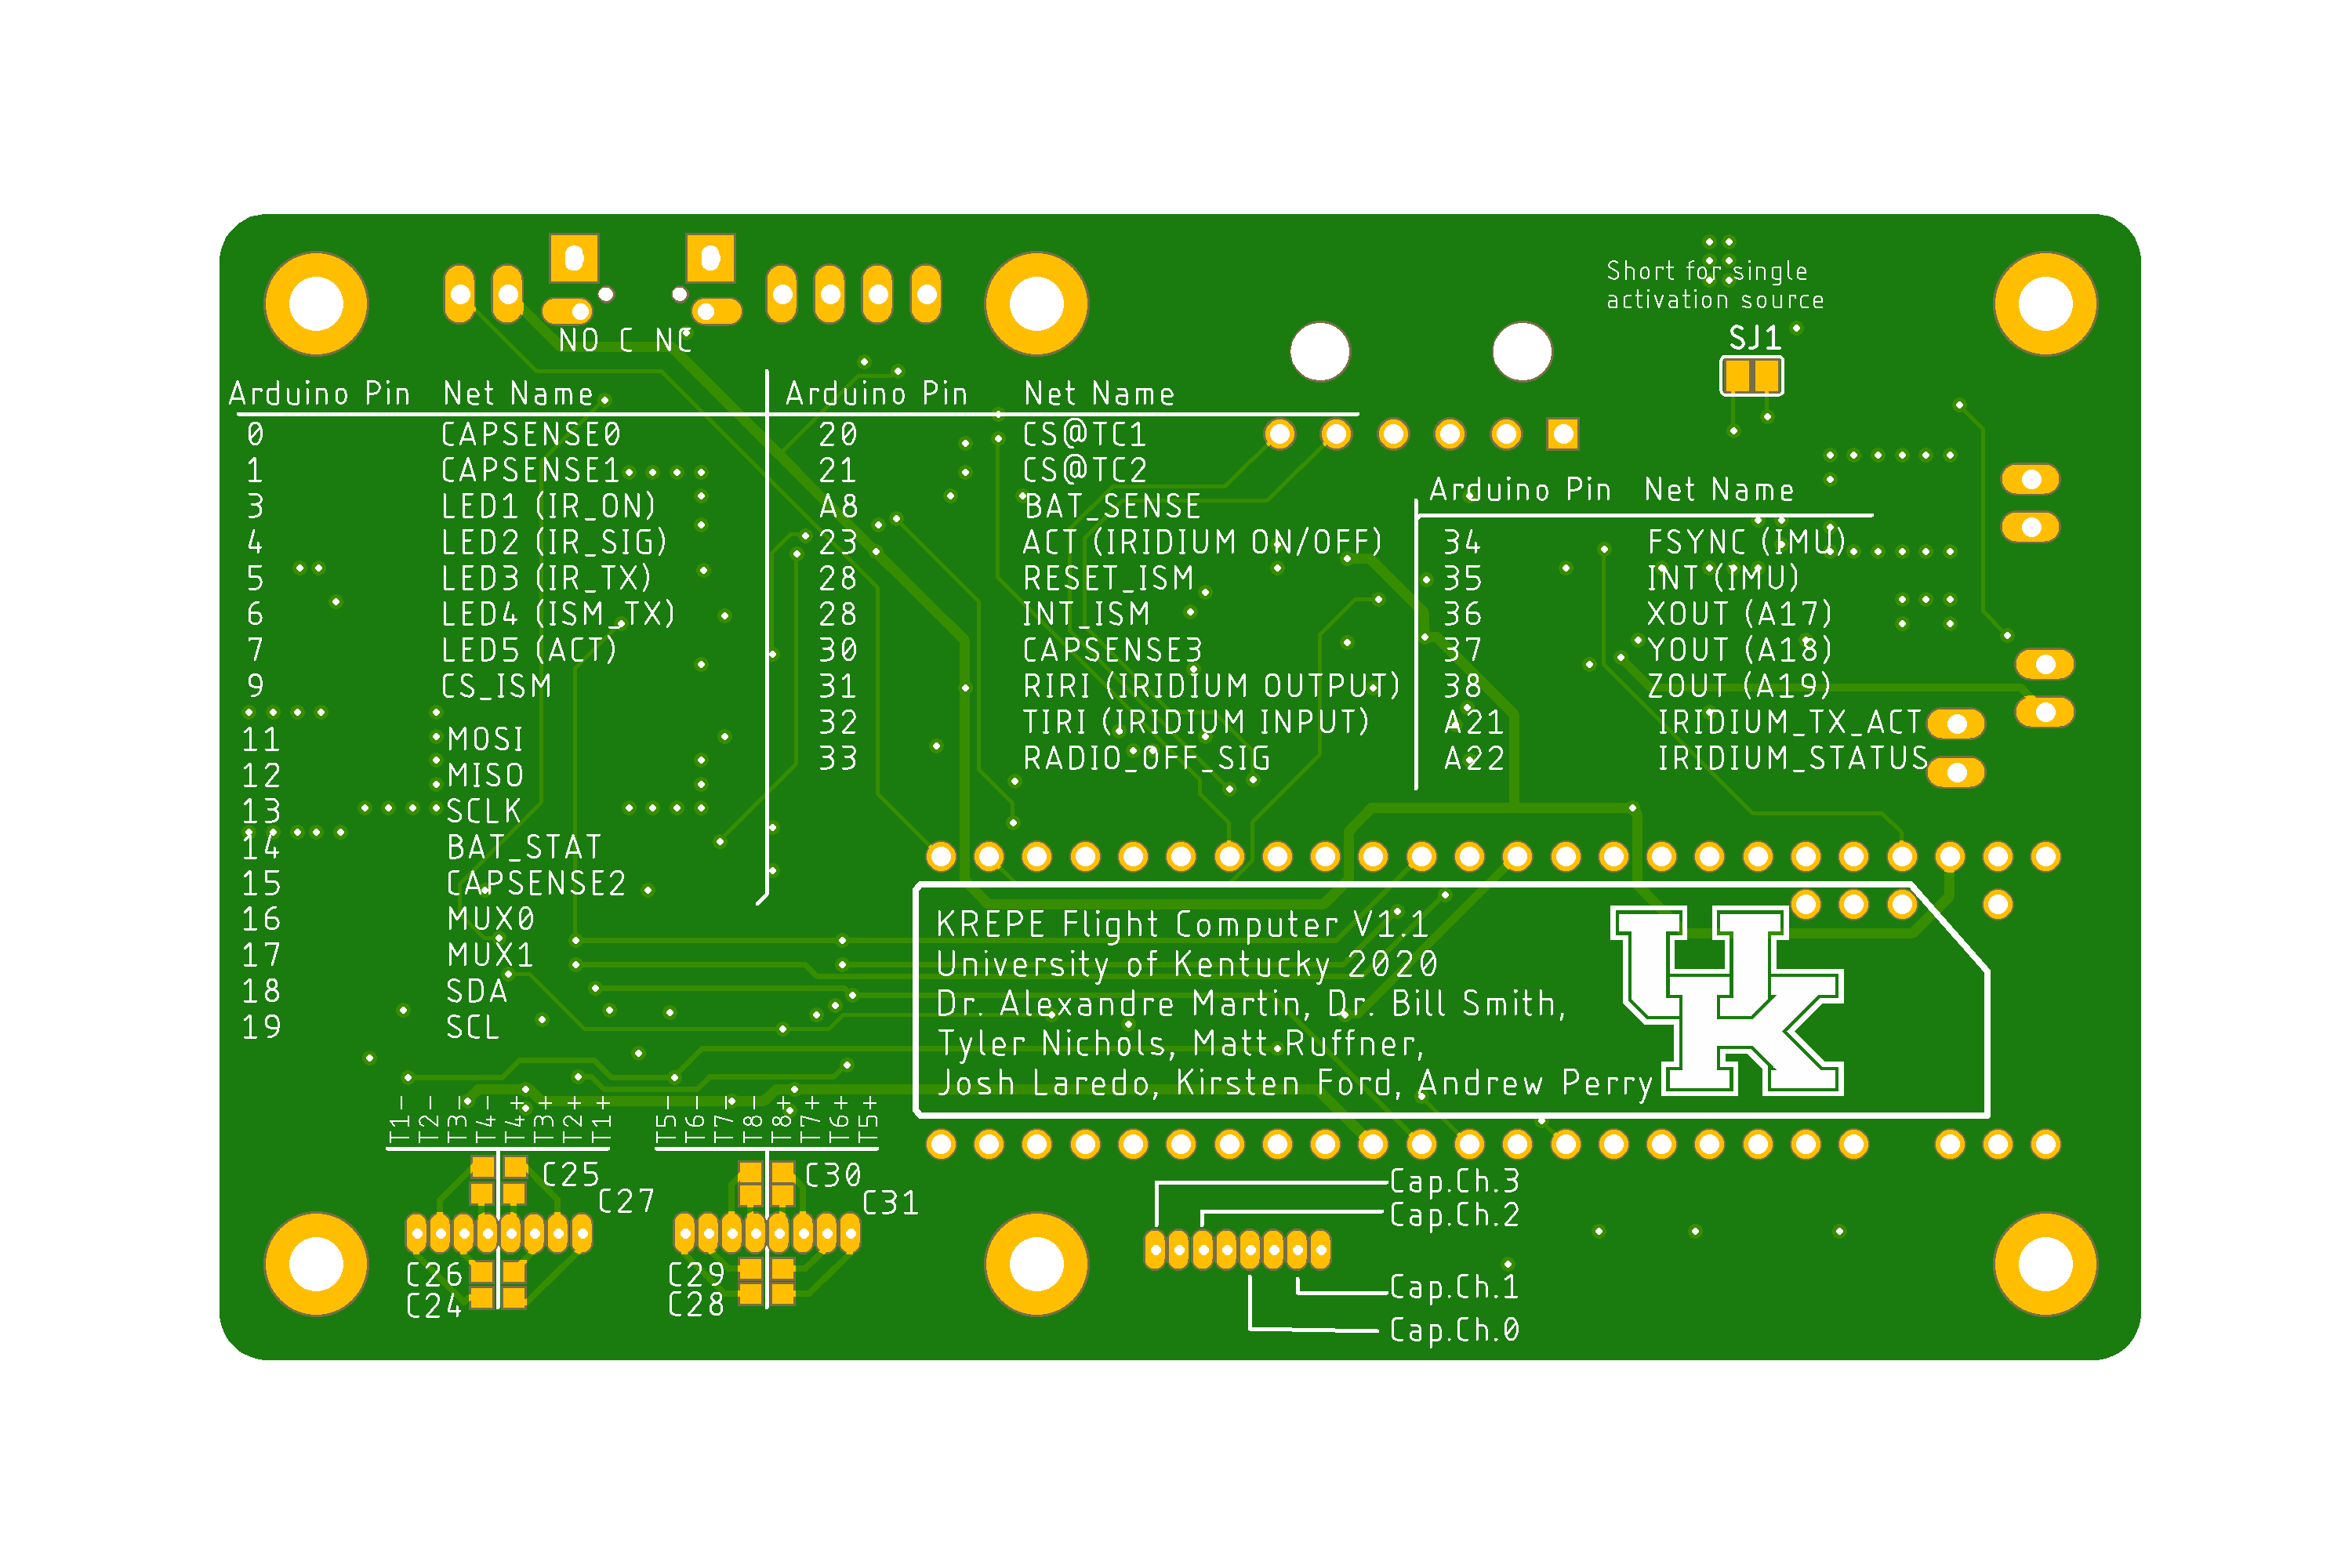
\includegraphics[width=\textwidth]{images/krepe-bottom.png}
    \caption{Rendering of the bottom of the KREPE control board, V1.1.}
    \label{fig:board-bottom}
\end{figure}

The \texttt{ISM\_SW} header is meant to enable and disable the RFM69 debug radio. The center 3.3V pin of this header is connected to the normally closed labeled pin, a GPIO pin is pulled high (see Fig. \ref{tab:pins_radio}). When the normally closed pin is connected to the center pin, the RFM69 is enabled. This way, debug communication can be used while testing in a way that also ensures it will be off when on a live mission. This radio is only used for ground testing communication purposes, and once handed over for final integration, will never be enabled or able to receive power. These\footnote{\url{https://www.digikey.com/product-detail/en/omron-electronics-inc-emc-div/D2SW-3L1H/Z12268-ND/1811989}} are the switches used for the pin pull activation.




\subsection{Secondary Activation}
Once primary activation is complete and the flight computer is in standby mode, sensors are polled to check for conditions necessary for secondary activation. Secondary activation is software based and only engaged once the KREPE probe has separated from its protective metal enclosure. No radio transmissions are attempted before secondary activation. 

Thermocouples and a capacitive sensing subsystem are polled to check for conditions sufficient for secondary activation. A heating of the metal KREPE enclosure is necessary to melt the plastic bolts that hold it together. This ambient temperature increase of the probe is the primary criteria for secondary activation. The presence of this metal enclosure is also detected by capacitive sensors on the KREPE probe. Once the thermal and capacitive sensing subsystems have detected the separation of the metal enclosure, the Iridium radio is powered on and packet transmission begins.  

\section{Subsystems}

\subsection{Status and Error Indicators}
\begin{table}[H]
    \centering
    \begin{tabular}{c|c|c}
    Teensy Pin & Net Name     & Teensy Configuration \\
    \hline 
    3 & LED1 - IRIDIUM ON        &   \texttt{OUTPUT}\\
    4 & LED2 - IRIDIUM SIGNAL OK       &   \texttt{OUTPUT}\\
    5 & LED3 - IRIDIUM RADIO TRANSMITTING       &   \texttt{OUTPUT}\\
    6 & LED4 - ISM RADIO TRANSMITTING       &   \texttt{OUTPUT}\\
    7 & LED5 - GENERAL ACTIVITY       &   \texttt{OUTPUT}
    \end{tabular}
    \caption{Debug LED Connections.}
    \label{tab:pins_leds}
\end{table}

\subsection{Serial Interface Signals}

\begin{table}[H]
    \centering
    \begin{tabular}{l|l|c}
   Teensy Pin & Net Name &  Description \\
    \hline \hline
    
        \hline
    13 & SCLK     &  SPI Clock \\
    12 & MISO     &  Master In Subject Out \\
    11 & MOSI     &  Master Out Subject In \\
    20 & CS@TC1 & U10 (MAX31855) chip select, active low \\
    21 & CS@TC2 & U11 (MAX31855) chip select, active low  \\
    9 & CS\_ISM     & RFM69 chip select, active low  \\
    \hline
    32 & TIRI     & Iridium TX UART \\
    31 & RIRI      & Iridium RX UART \\
    \hline
    19 & SCL & I$^2$C bus clock \\
    18 & SDA & I$^2$C bus data
    \end{tabular}
    \caption{Pins used with SPI, I$^2$C, and UART interfaces.}
    \label{tab:pins_serial}
\end{table}

\subsection{RFM69 Radio}
Note that this radio is not supplied with power unless the \texttt{NO} to \texttt{C} connection is made on the \texttt{ISM\_SW} header (see Fig. \ref{fig:board-top}).  Maximum output power according to the radio datasheet (\url{https://cdn.sparkfun.com/datasheets/Wireless/General/RFM69HCW-V1.1.pdf}) is 100mW.
\begin{table}[H]
    \centering
    \begin{tabular}{c|c|c|r}
    Teensy Pin & Net Name  & Description   & Teensy Configuration \\
    \hline 
    28 & RESET\_ISM  &  Pull low to enable RFM69   & \texttt{OUTPUT} \\
    29 & INT\_ISM    &  GPIO0 interrupt from RFM69 & \texttt{INPUT} \\
    33 & RADIO\_OFF\_SIG & Pulled high when the RFM69 is disabled & \texttt{INPUT} \\
    \end{tabular}
    \caption{Radio module interface signals.}
    \label{tab:pins_radio}
\end{table}
The datasheet for this antenna can be found at  \url{https://cdn.taoglas.com/datasheets/FXP290.07.0100A.pdf}. 

\subsection{Iriduim Radio}
We are using the A3LA-RS type modem seen on the NAL Research site (\url{http://www.nalresearch.com/IridiumHardware.html}). The RF specifications, taken from the module's datasheet are shown in Fig. \ref{fig:iridium-rf-specs}.

\begin{figure}[H]
    \centering
    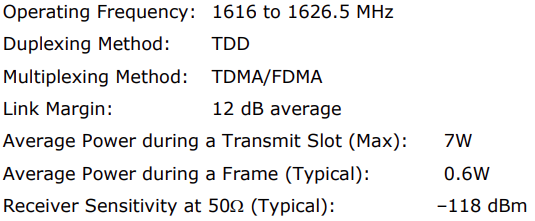
\includegraphics[width=0.5\textwidth]{images/iridium-rf-specs.png}
    \caption{RF specifications of the AL3A-RS Iridium modem.}
    \label{fig:iridium-rf-specs}
\end{figure}
  
\subsubsection{Radio Power Control}
\begin{table}[H]
    \centering
    \begin{tabular}{l|l|c|r}
   Teensy Pin & Net Name     &  Description  & Teensy Configuration \\
    \hline
    23 & ACT   & Iridium activation, active high & \texttt{OUTPUT} \\
    \end{tabular}
    \caption{Pin controlling power to the iridium satellite radio.}
    \label{tab:pins_iridium}
\end{table}

\subsection{Thermocouple Measurement Interface}
Note: this board features an update thermocouple interface IC than the previous boards. Among other enhancements it allows for broader temperature range reading and improved precision.
\begin{table}[H]
    \centering
    \begin{tabular}{c|c|c|r}
    Teensy Pin & Net Name  & Description   & Teensy Configuration \\
    \hline 
    16 & MUX0 & IC1 and IC2 mux. select pin & \texttt{OUTPUT} \\
    17 & MUX1 & IC1 and IC2 mux. select pin & \texttt{OUTPUT} \\ 
    \end{tabular}
    \caption{Analog mux selection pins.}
    \label{tab:pins_thermo}
\end{table}

\subsubsection{Thermocouple Connections}
See datasheet and connections in the relevant schematics in Fig. \ref{fig:page1_1} in Appendix \ref{appa}.

TODO: image of connector placements on board to facilitate wiring of a new connector.


\subsection{Motion Sensor Connections}

\begin{table}[H]
    \centering
    \begin{tabular}{c|c|c|r}
    Teensy Pin & Net Name  & Description   & Teensy Configuration \\
    \hline 
    36 A17 & XOUT & Analog out from accel (x axis) & \texttt{INPUT} \\
    37 A18 & YOUT & Analog out from accel (y axis) & \texttt{INPUT} \\
    38 A19 & ZOUT & Analog out from accel (z axis) & \texttt{INPUT} \\
    35 & INT & Interrupt from ICM-20948 & \texttt{INPUT} \\
    34 & FSYNC & Synchronization signal to ICM-20948 & \texttt{OUTPUT} 
    \end{tabular}
    \caption{Pins connecting to the ADXL377 and ICM-20948.}
    \label{tab:pins_motionsensor}
\end{table}



\subsection{Charging and Power}

Charge current is limited to to 450 mA. Charge power can be delivered via Teensy USB or the \texttt{CHARGE} header. Charging input voltage is expected to be 5 volts.

For battery protection, the adafruit batteries we use (\url{https://www.adafruit.com/product/354}) have built in protection circuitry. Charge management is handled by an MCP73831 IC (\url{https://www.microchip.com/wwwproducts/en/MCP73831}), with status connections to the Teensy as shown in Table \ref{tab:pins_battery}. Schematics and electrical connections are shown in Fig. \ref{fig:page1_3} in Appendix \ref{appa}.

\subsubsection{Battery Status Interface}
\begin{table}[H]
    \centering
    \begin{tabular}{c|c|c|r}
    Teensy Pin & Net Name  & Description   & Teensy Configuration \\
    \hline 
    14 & BAT\_STAT & LiPo charge state & \texttt{OUTPUT} \\
    22 A8 & BAT\_SENSE    &  Halved battery voltage for monitoring &   \texttt{INPUT} \\
    \end{tabular}
    \caption{Pins to monitor battery voltage and charging status.}
    \label{tab:pins_battery}
\end{table}

\subsubsection{Battery Protection}
Protection circuitry is implemented on the flight board to support 2P1S LiPo packs for system power. We are using a TI BQ2970 Voltage and Current Protection IC (\url{ http://www.ti.com/lit/ds/symlink/bq2970.pdf}). Protection circuitry as implemented on the KREPE flight computer PCB is shown in Fig. \ref{fig:bat-protec}.

\begin{figure}[H]
    \centering
    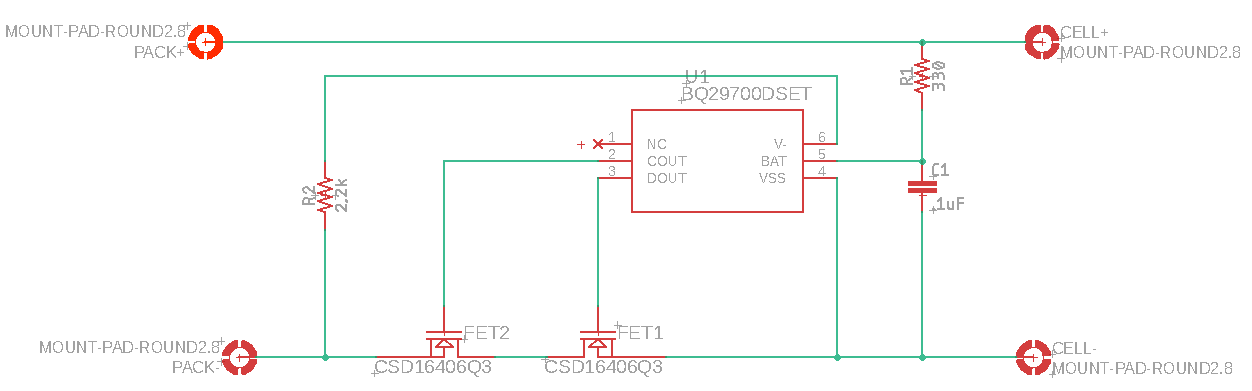
\includegraphics[width=\textwidth]{images/battery_protection_schematic.png}
    \caption{Battery protection circuitry. Cell+ and Cell- attach to the battery pack and Pack+/Pack- face system power. This protection circuitry is upstream of the primary activation switch.}
    \label{fig:bat-protec}
\end{figure}

Renderings of the bottom and top of the battery protection PCB can be seen in Figs \ref{fig:bat-top} and \ref{fig:bat-bottom}.


\begin{figure}[H]
    \centering
    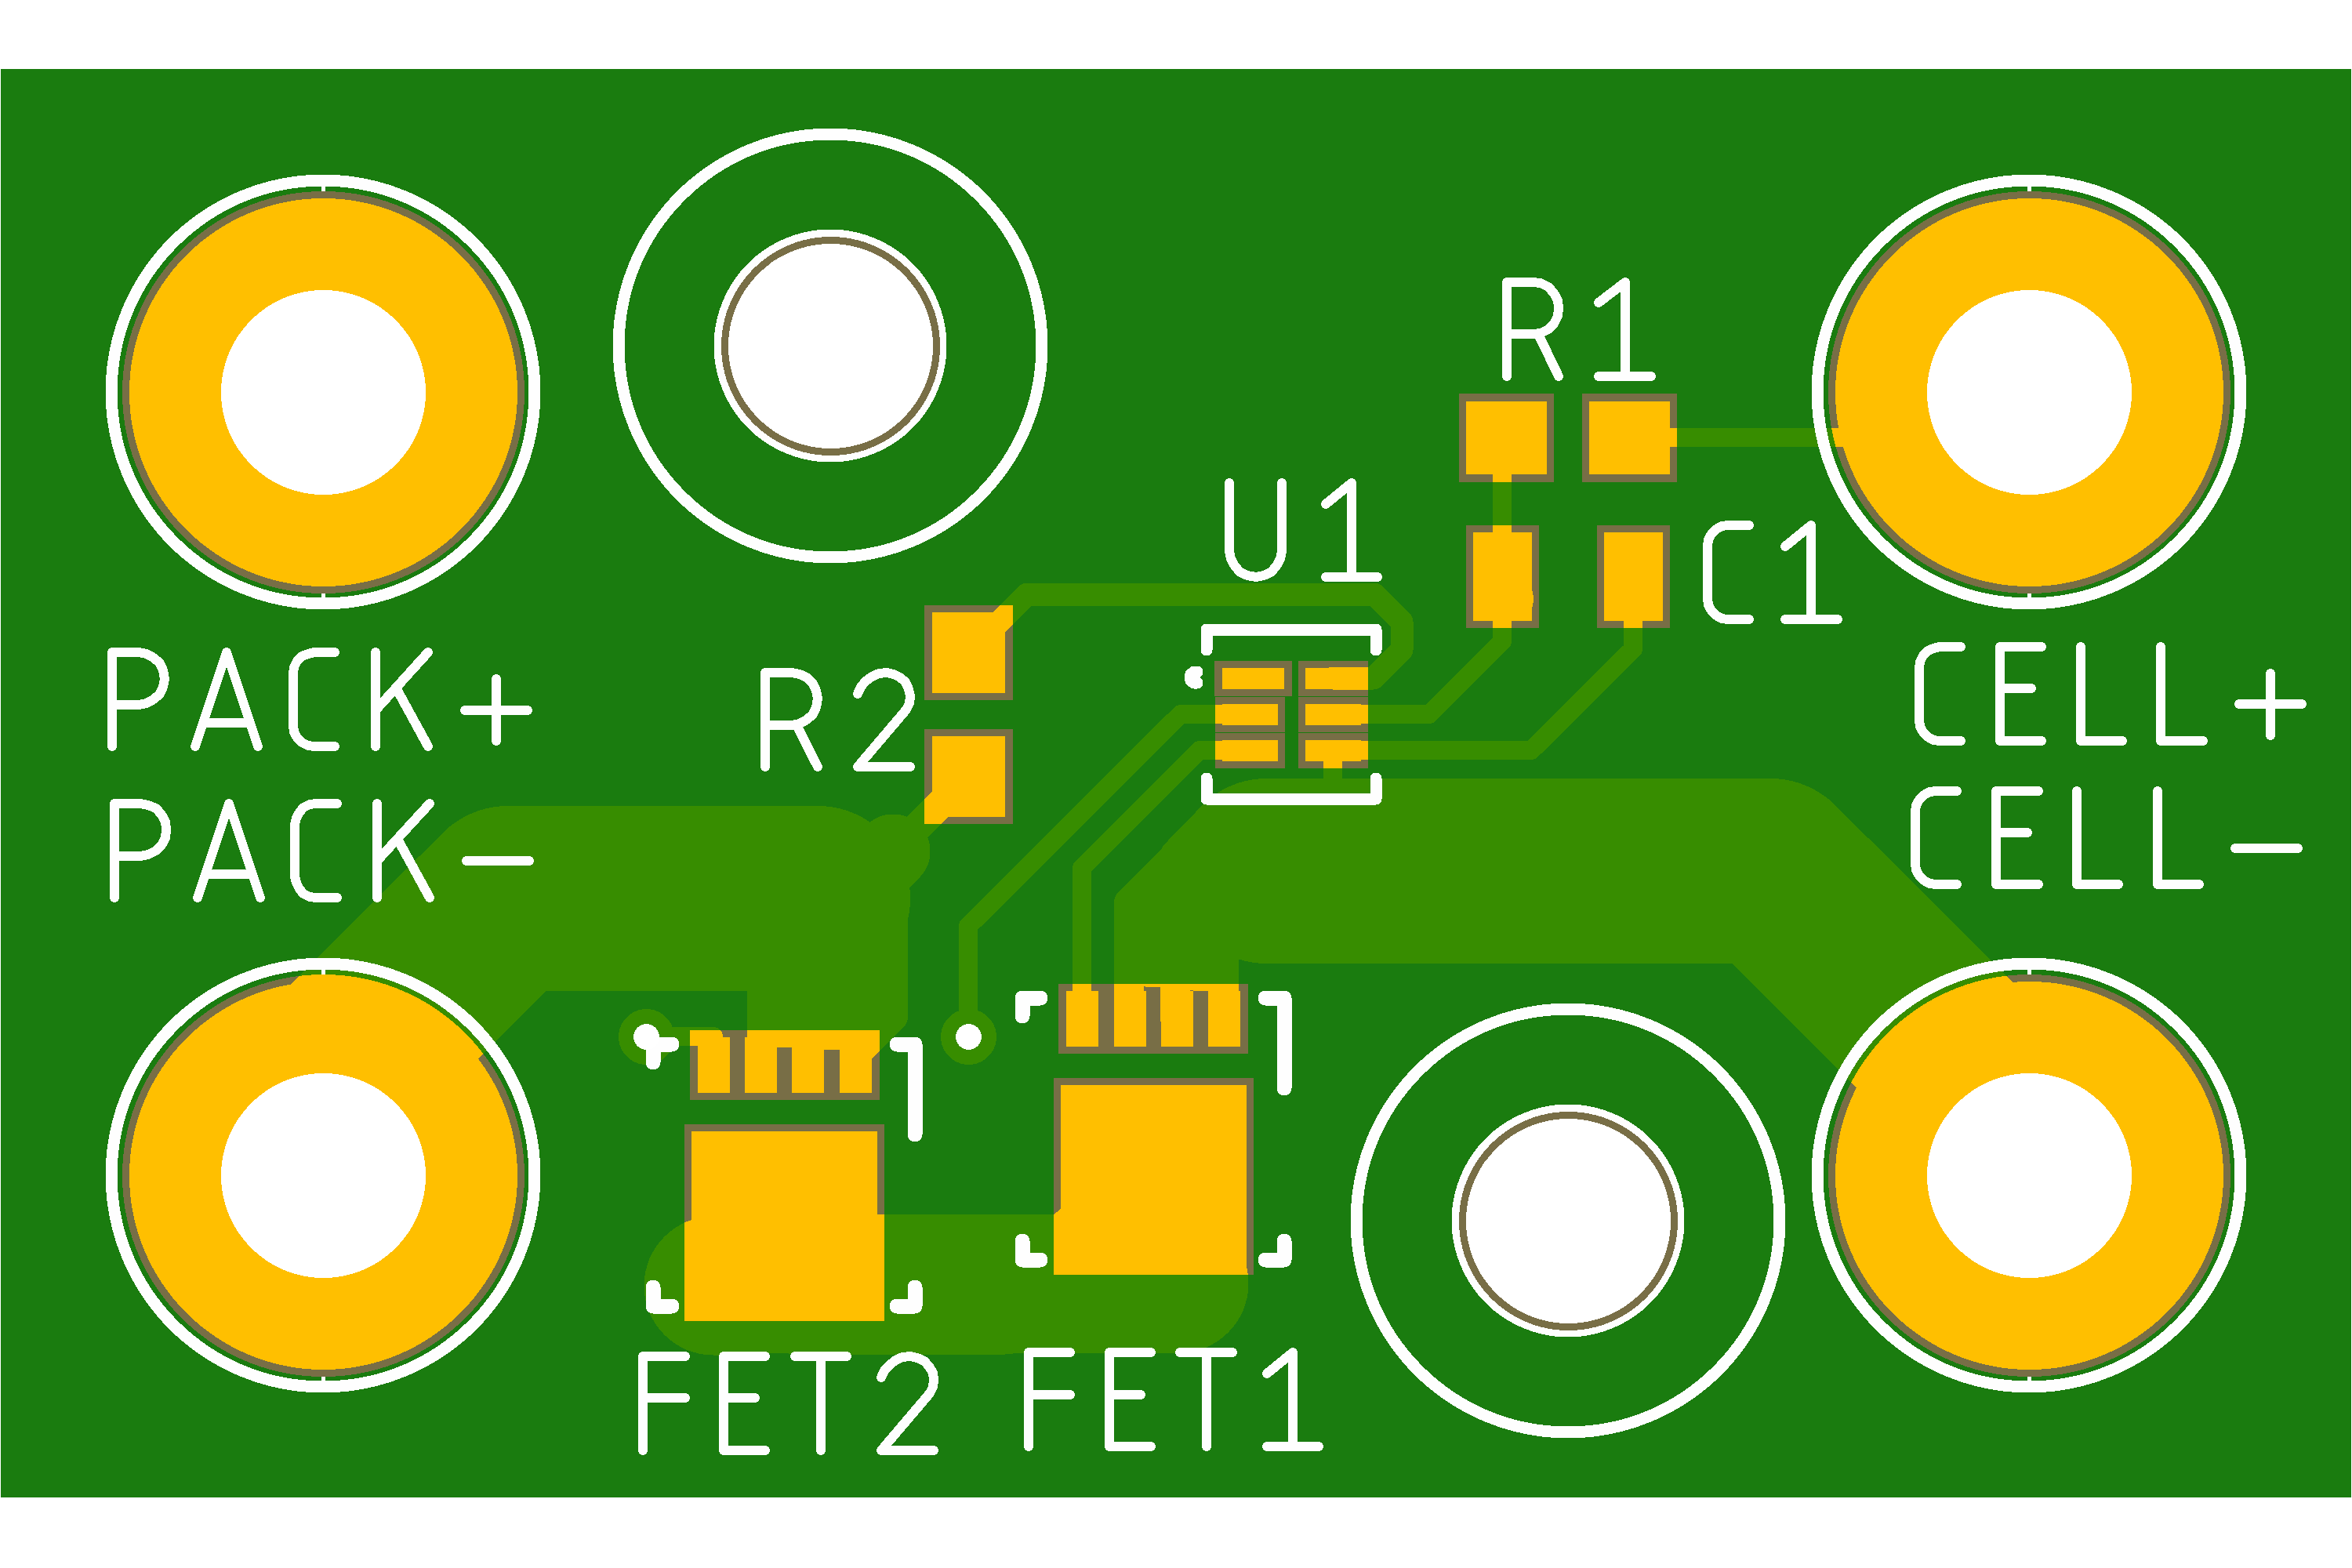
\includegraphics[width=0.4\textwidth]{images/BatteryProtection-render-top.png}
    \caption{Rendering of the top of the battery protection PCB.}
    \label{fig:bat-top}
\end{figure}


\begin{figure}[H]
    \centering
    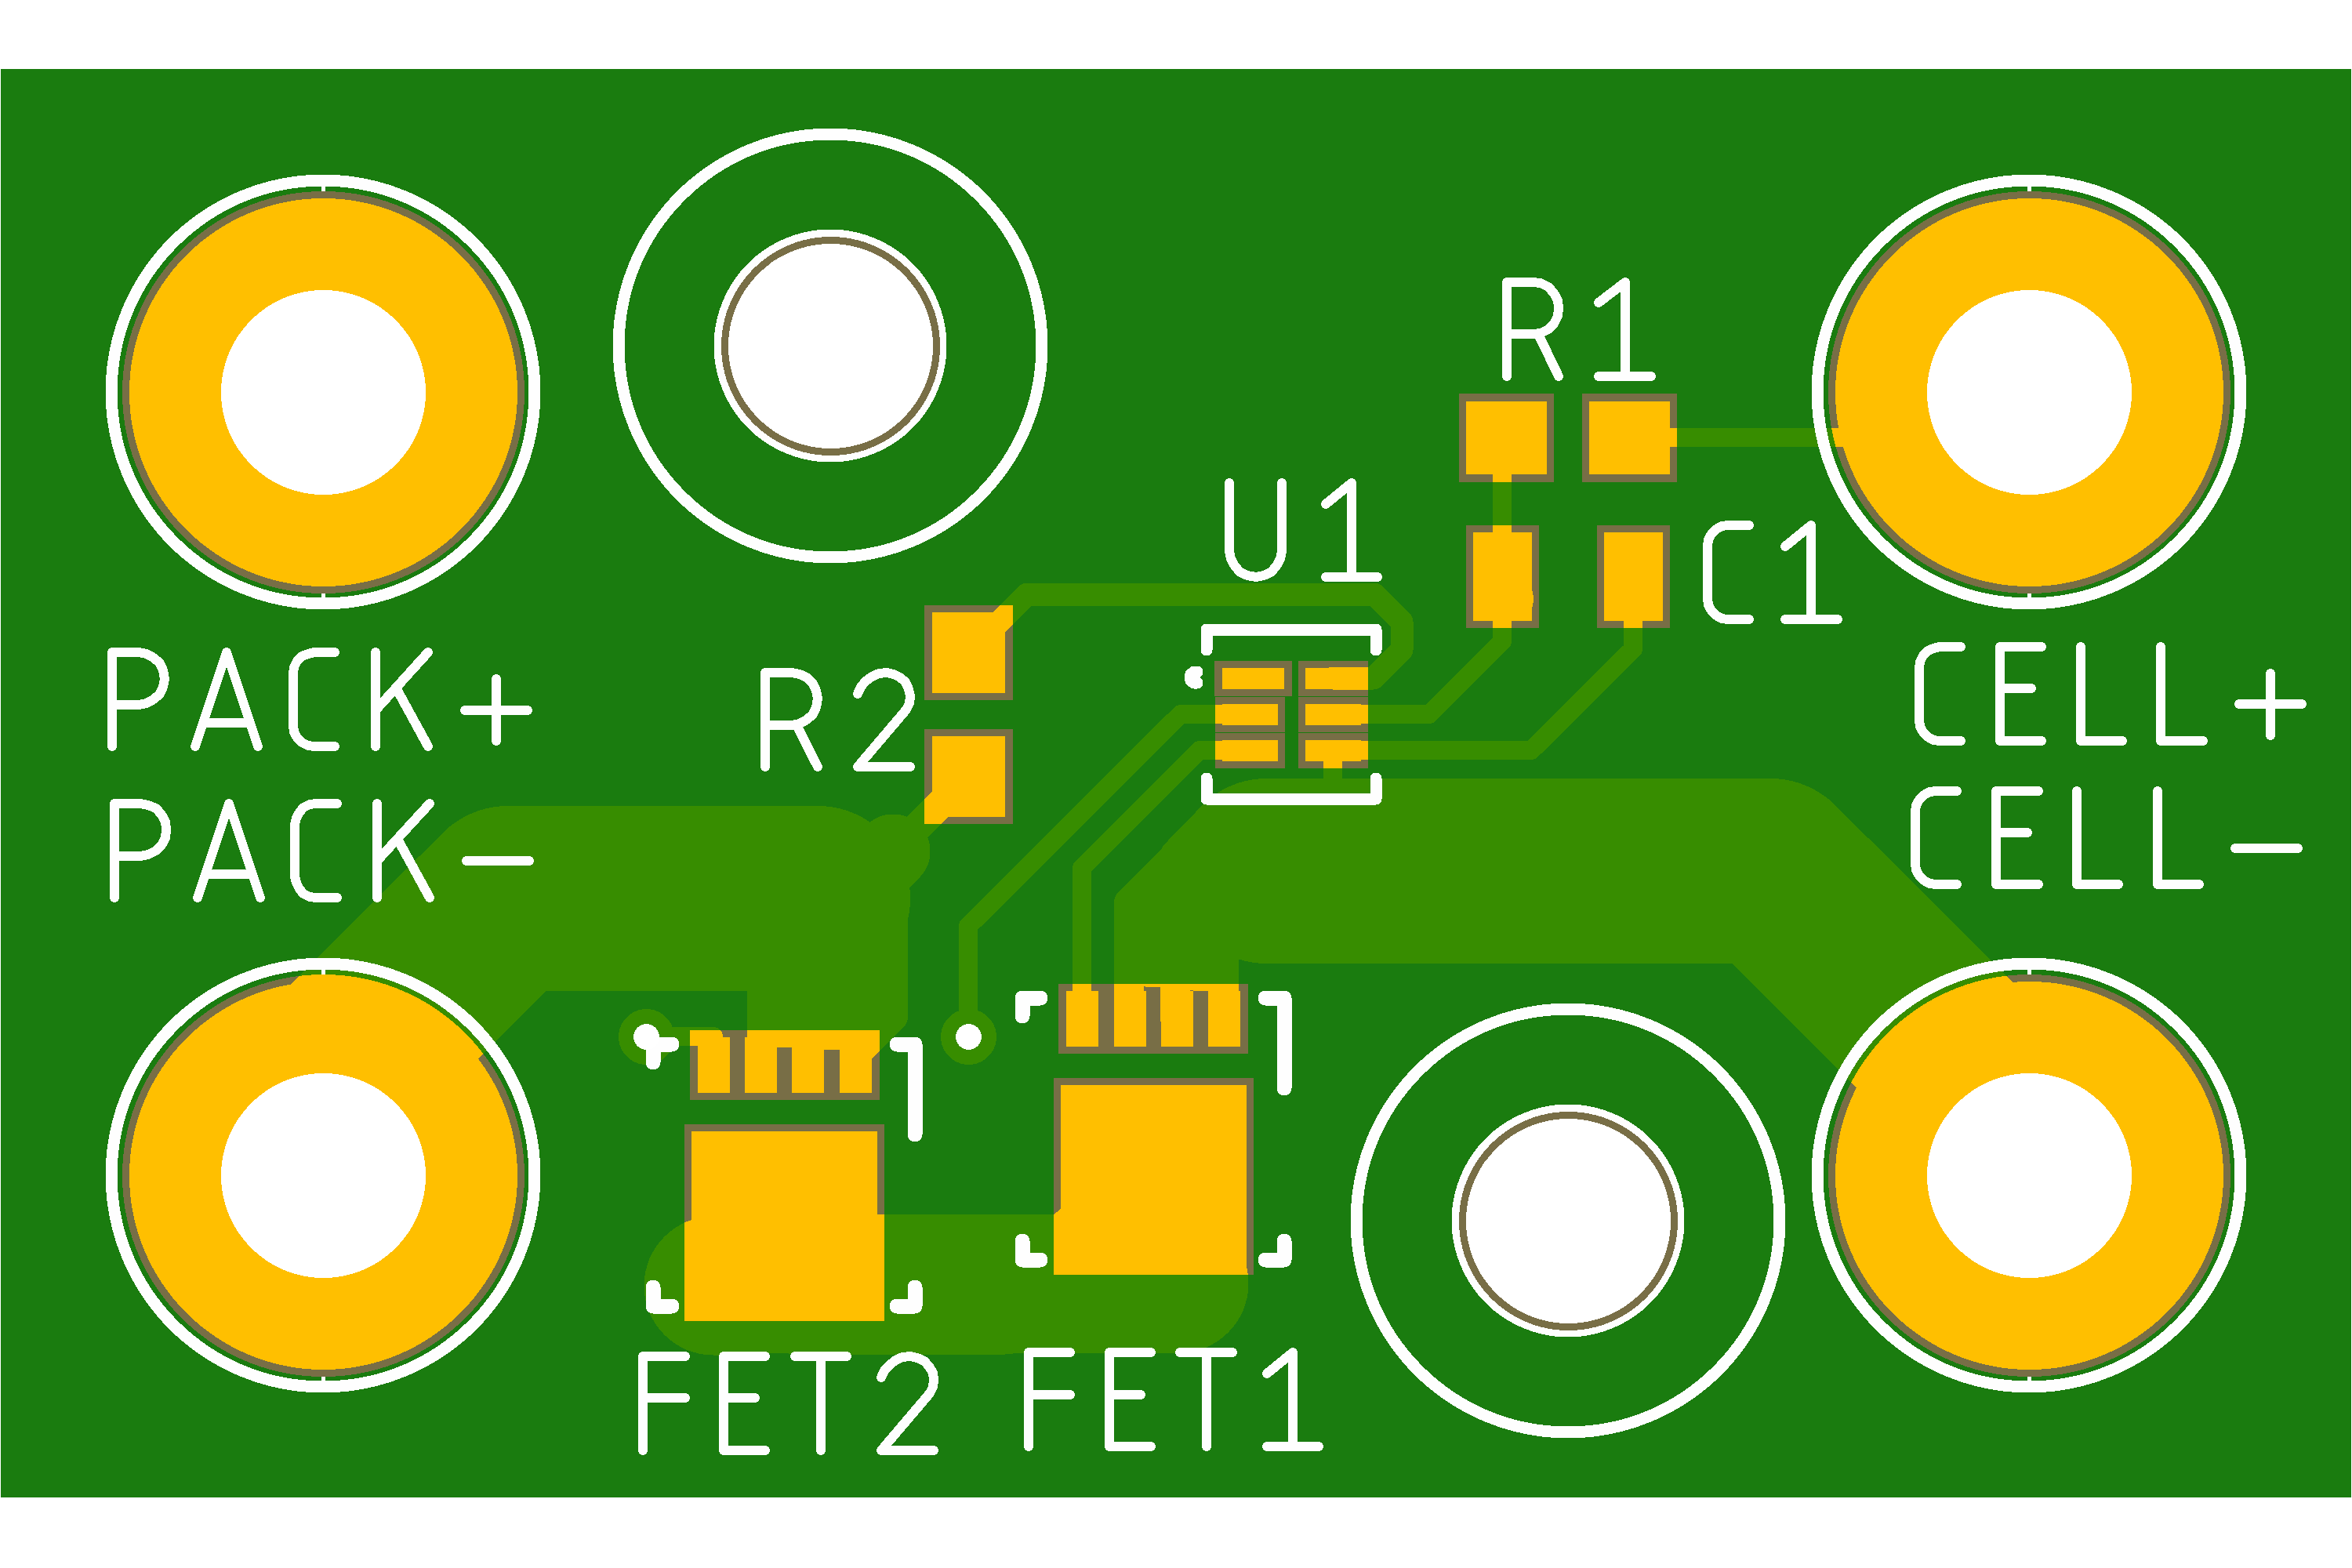
\includegraphics[width=0.4\textwidth]{images/BatteryProtection-render-top.png}
    \caption{Rendering of the bottom of the battery protection PCB.}
    \label{fig:bat-bottom}
\end{figure}

\section{Testing Software}

ICM-20948 testing software is functional. ADXL377 test software is functional. Lipo charge circuitry is functional. Need to test thermocouple hardware still.

TODO: simple sketch that tests a newly assembled board to make sure the IMU, accel, debug radio, iridium radio and thermocouple amplifiers are working as expected. 

























%%%%%%%%%%%%%%%%%%%%%%%%%%%%%%%%%%%%%%%%%%%%%%%%%%%%%%%%%%%%%%%%%%%%%%%%%%%%%%%%%%%
%%%%%%%%%%%%%%%%%%%%%%%%%%%%%%%%%%%%%%%%%%%%%%%%%%%%%%%%%%%%%%%%%%%%%%%%%%%%%%%%%%%
%%%%%%%%%%%%%%%%%%%%%%%%%%%%%%%%  APPENDIX
%%%%%%%%%%%%%%%%%%%%%%%%%%%%%%%%%%%%%%%%%%%%%%%%%%%%%%%%%%%%%%%%%%%%%%%%%%%%%%%%%%%
%%%%%%%%%%%%%%%%%%%%%%%%%%%%%%%%%%%%%%%%%%%%%%%%%%%%%%%%%%%%%%%%%%%%%%%%%%%%%%%%%%%
\appendix


\section{Schematics}
\label{appa}

\begin{figure}[H]
    \centering
    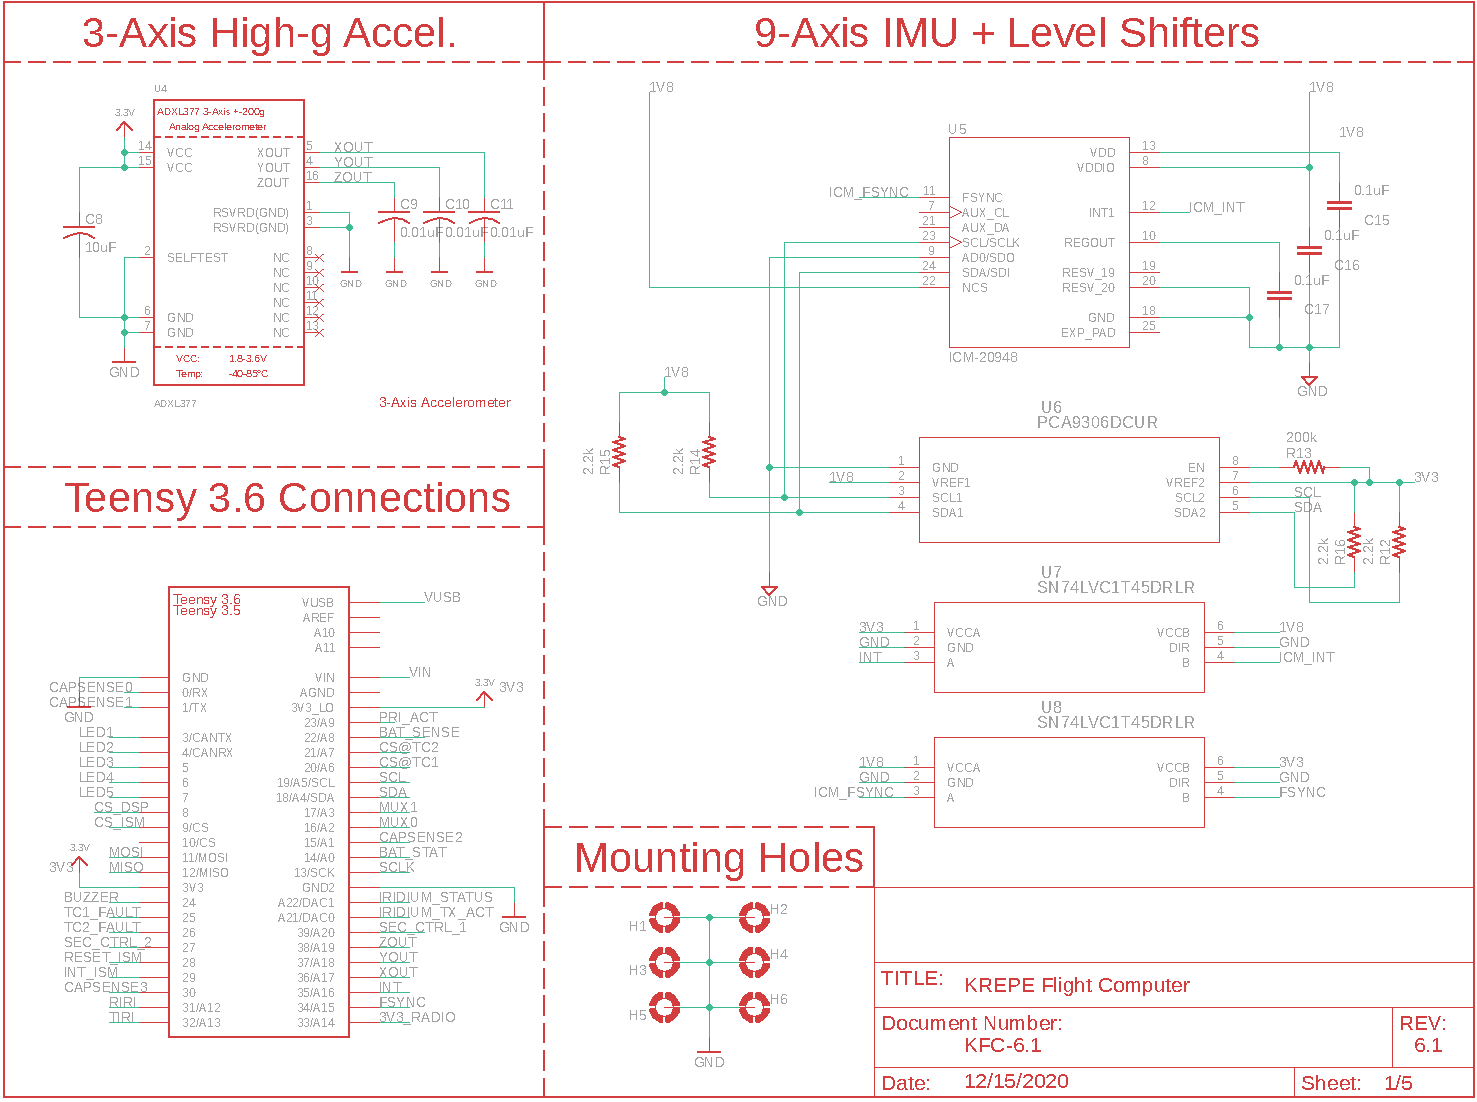
\includegraphics[width=\textwidth]{images/page1.png}
    \caption{Page one of schematics.}
    \label{fig:page1_2}
\end{figure}

\begin{figure}[H]
    \centering
    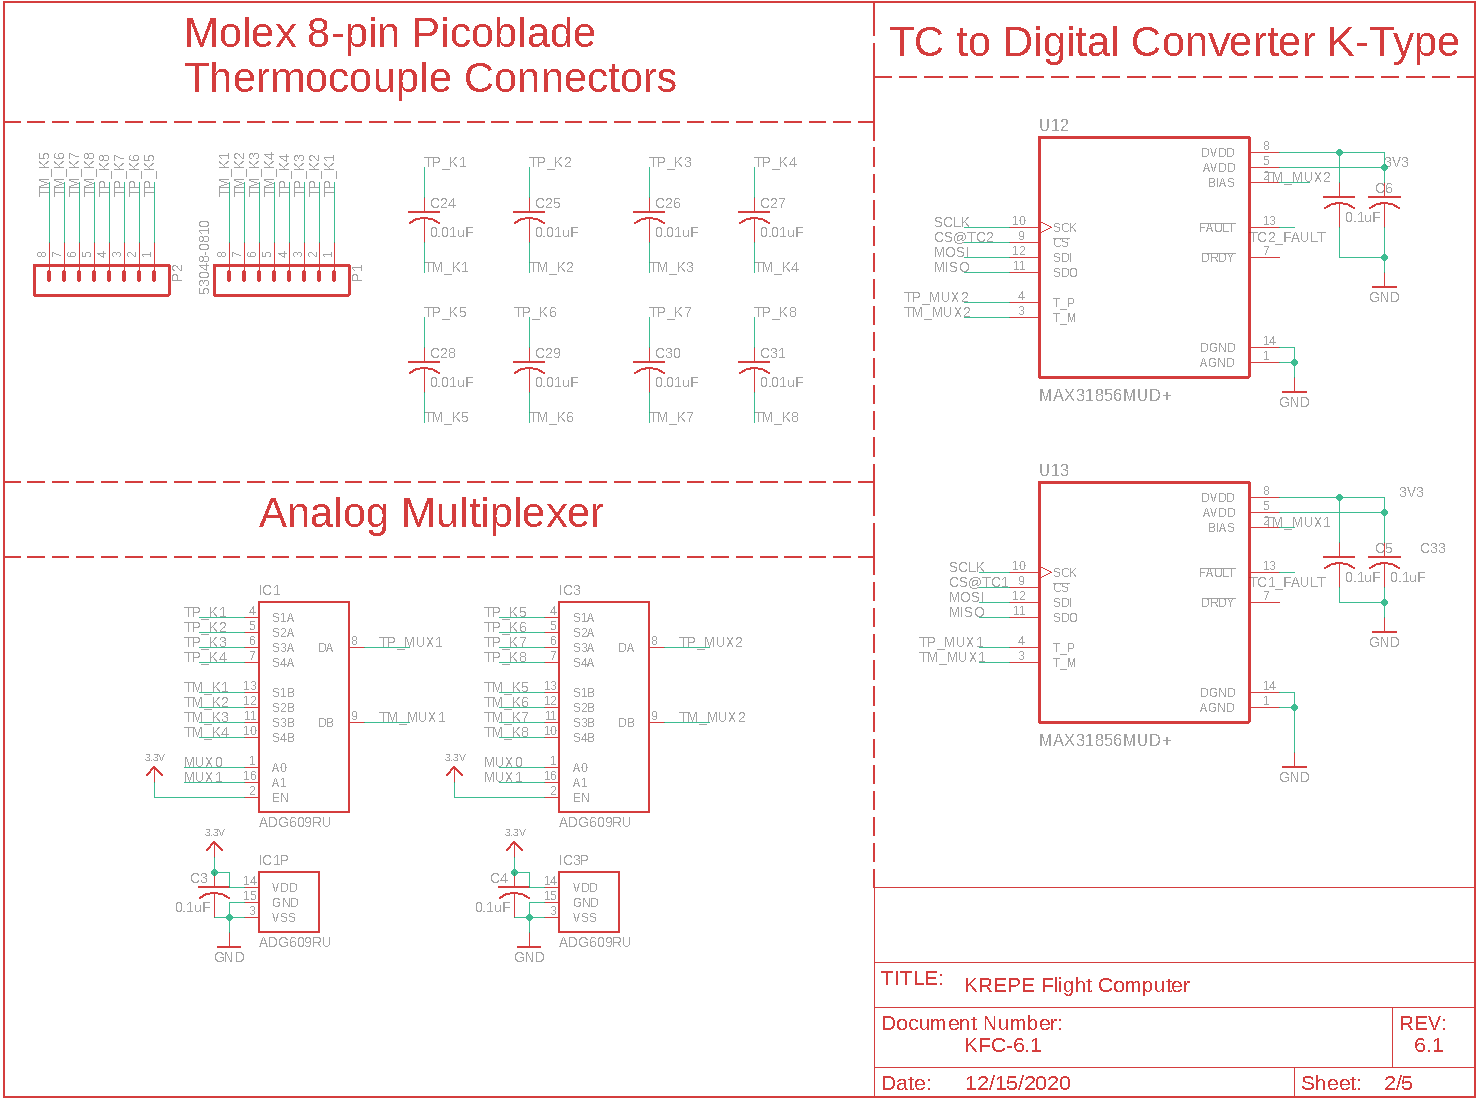
\includegraphics[width=\textwidth]{images/page2.png}
    \caption{Page two of schematics.}
    \label{fig:page1_1}
\end{figure}

\begin{figure}[H]
    \centering
    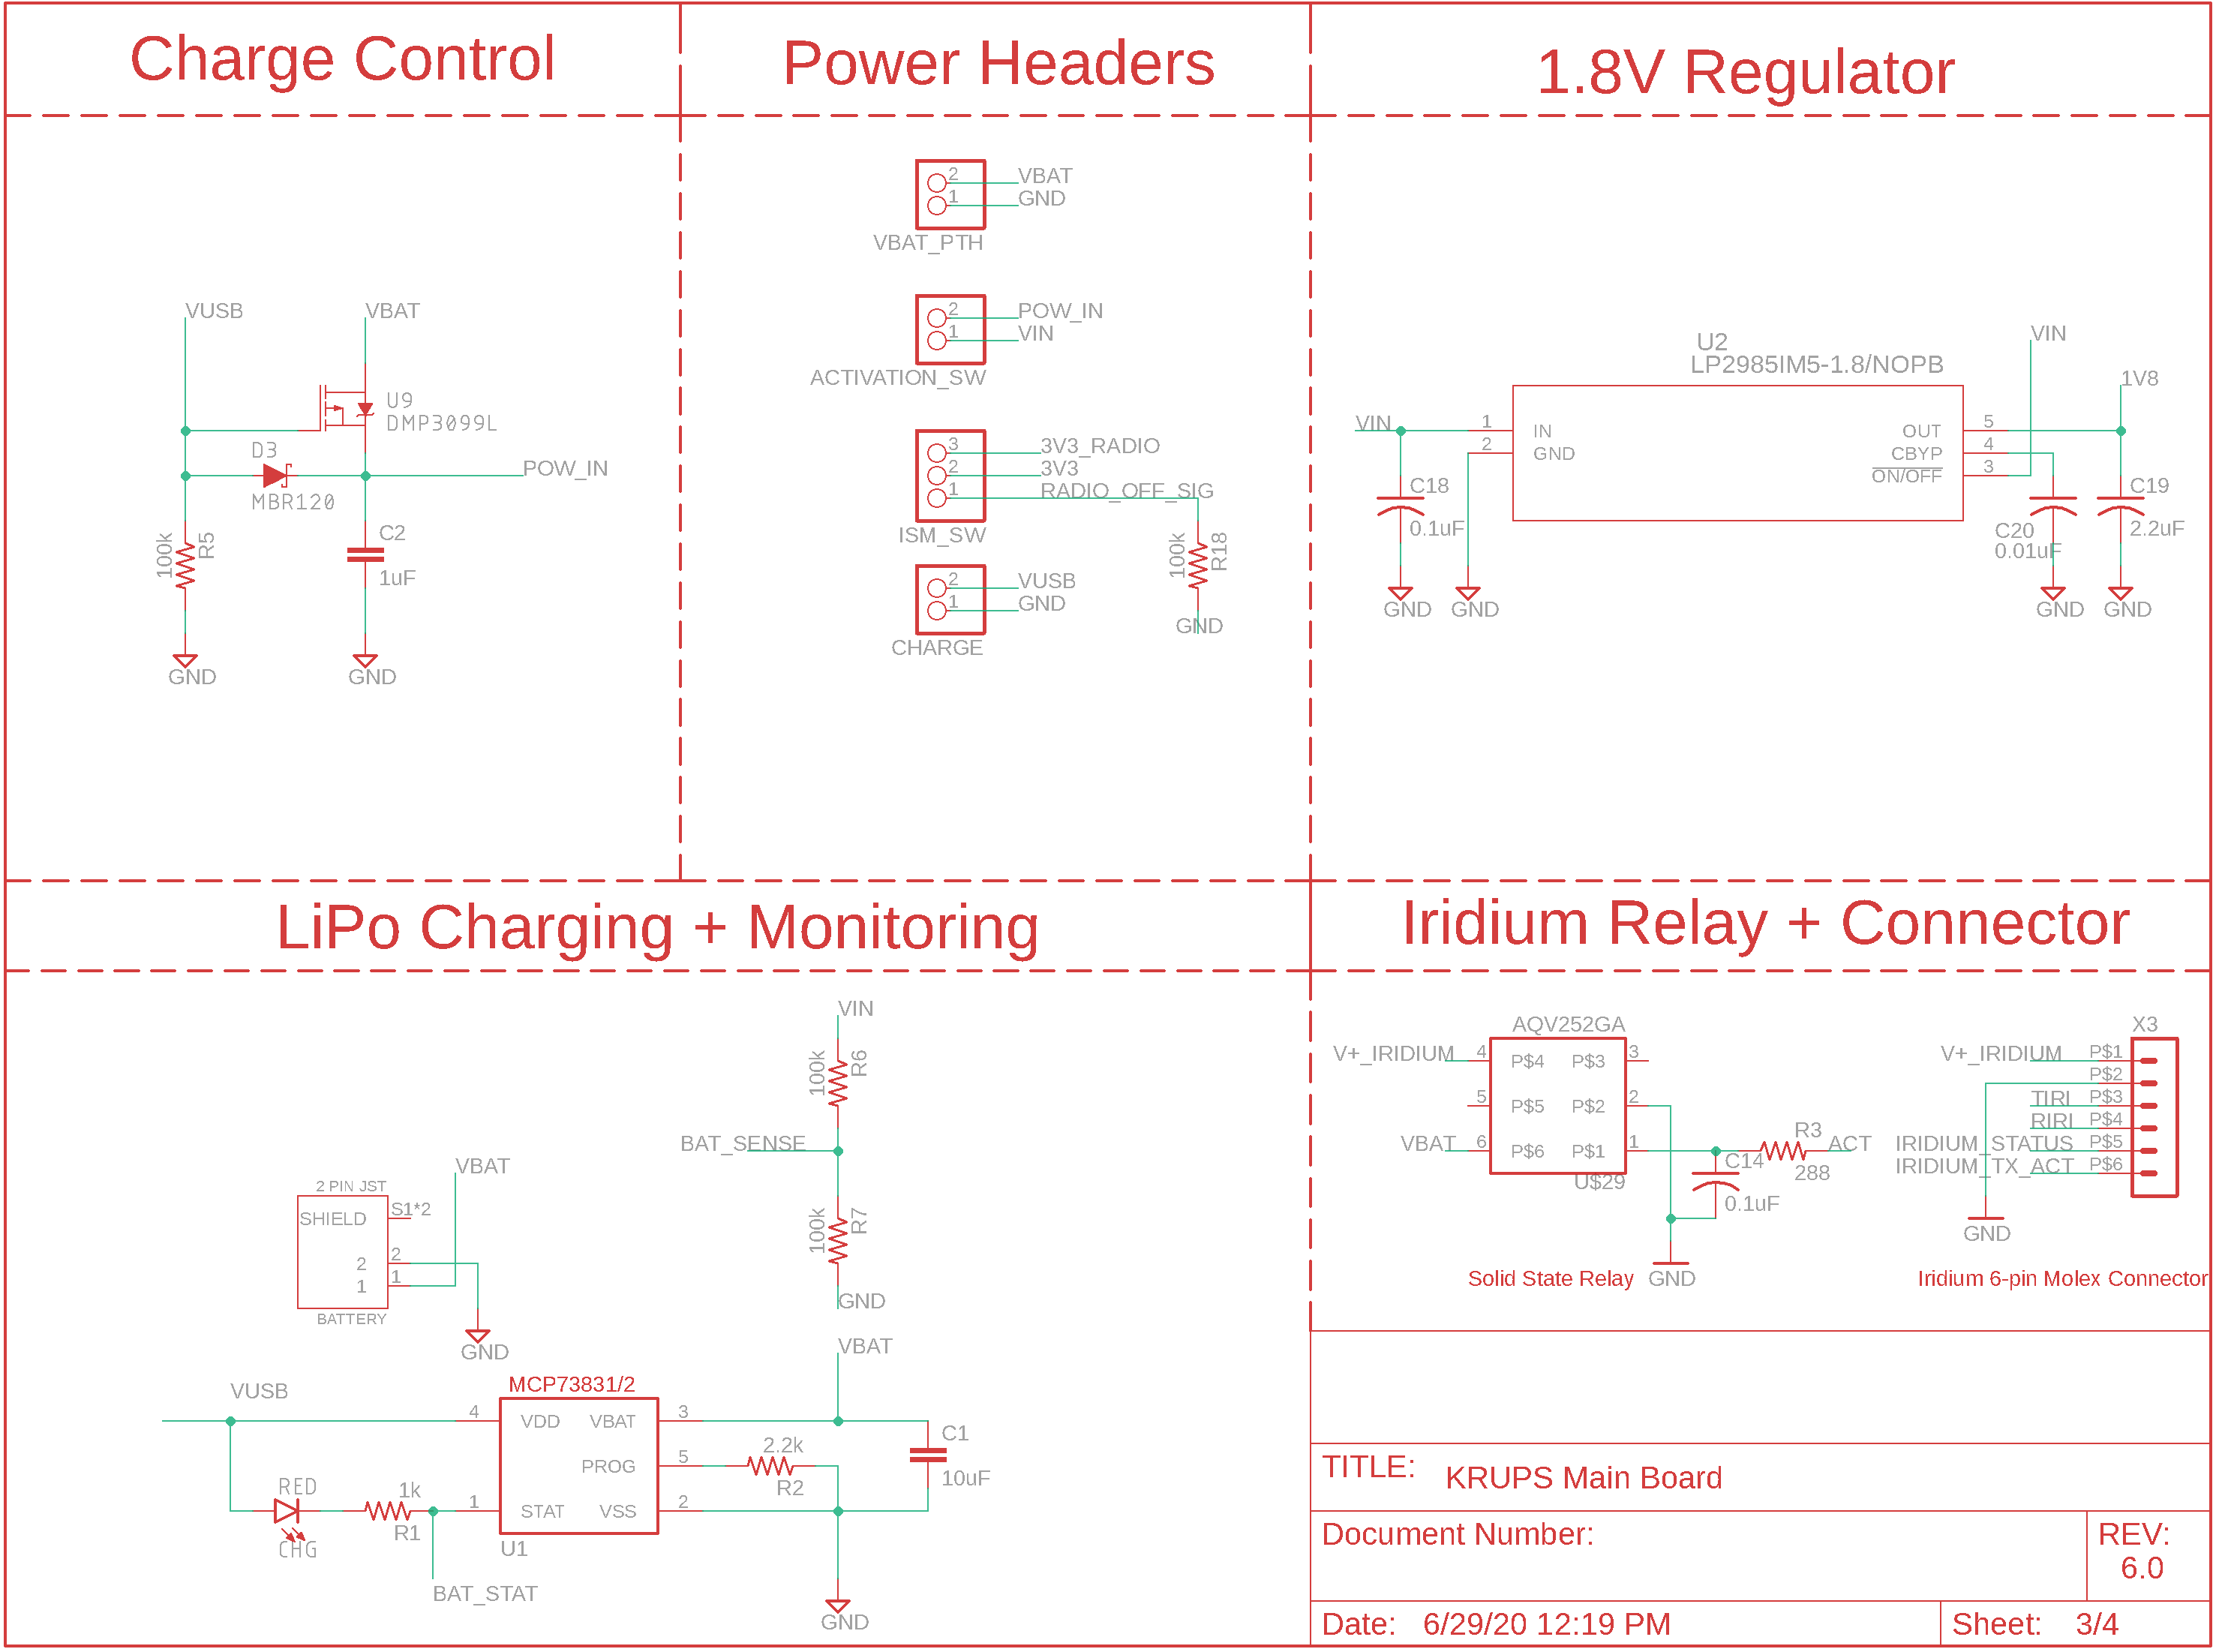
\includegraphics[width=\textwidth]{images/page3.png}
    \caption{Page three of schematics.}
    \label{fig:page1_3}
\end{figure}

\begin{figure}[H]
    \centering
    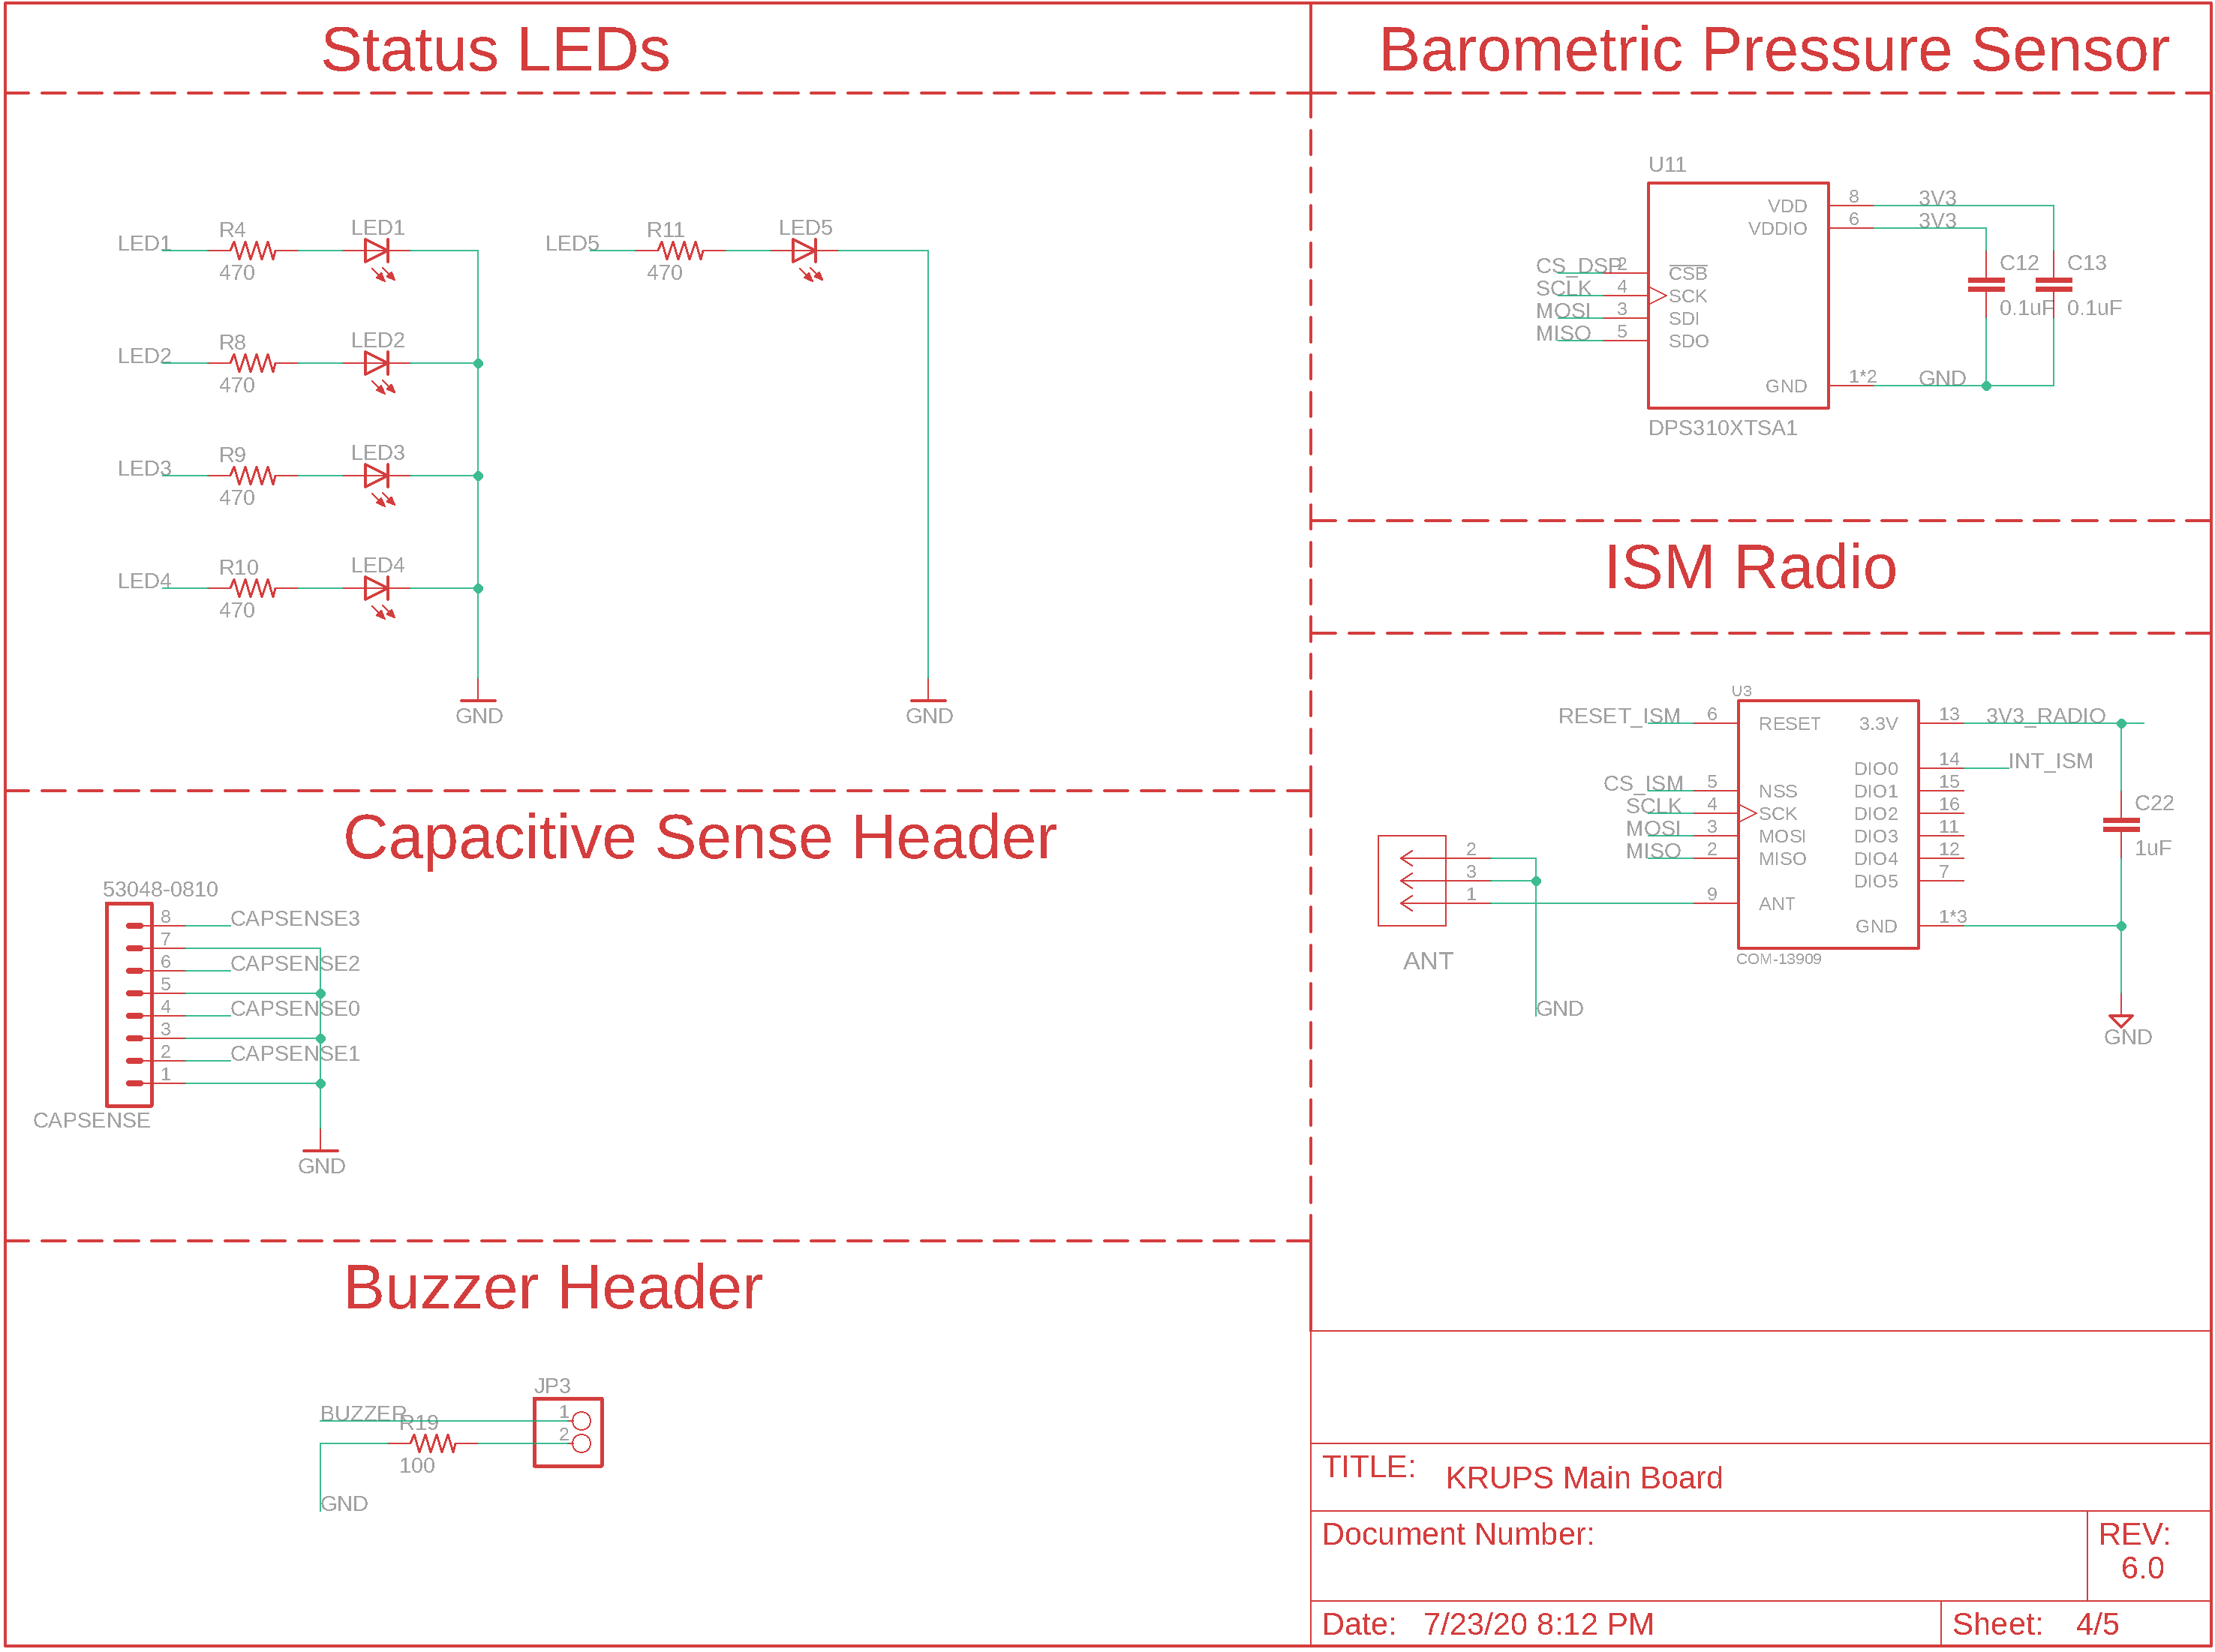
\includegraphics[width=\textwidth]{images/page4.png}
    \caption{Page four of schematics.}
    \label{fig:page1_4}
\end{figure}


\section{Teensy 3.5 Reference}

\begin{figure}[H]
    \centering
    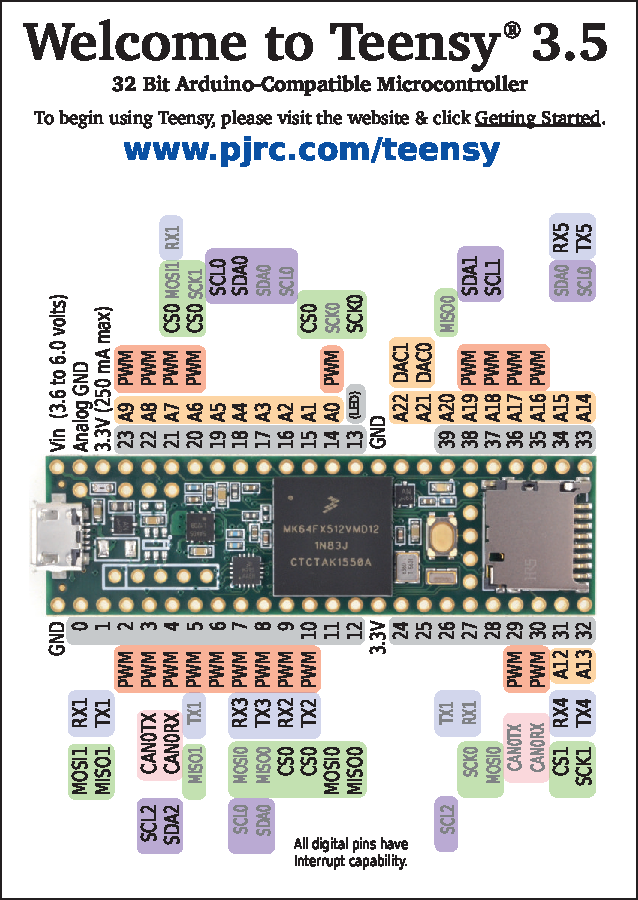
\includegraphics[width=\textwidth]{images/card8a_rev2.pdf}
    \caption{Teensy 3.5 Front}
    \label{fig:teensy_front}
\end{figure}

\begin{figure}[H]
    \centering
    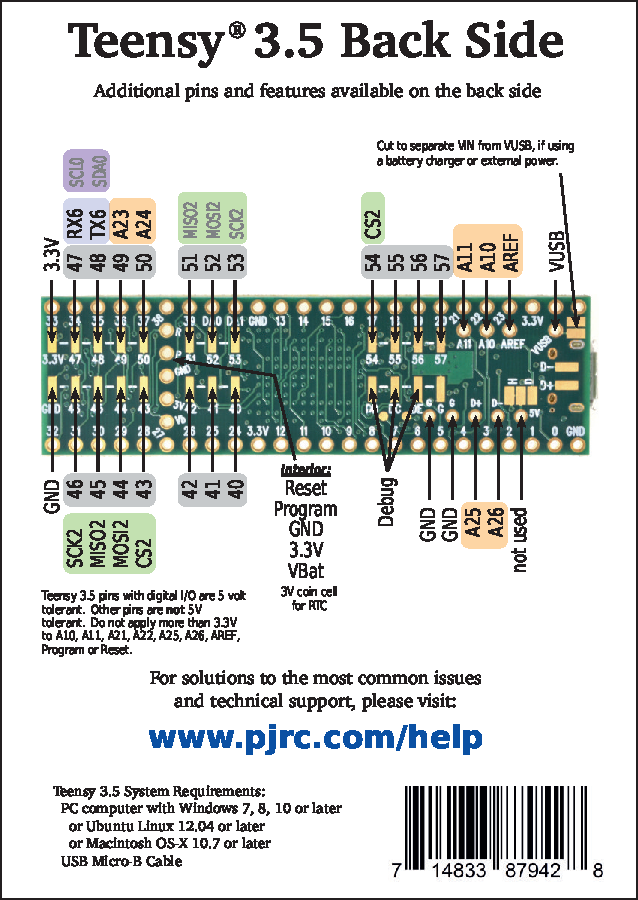
\includegraphics[width=\textwidth]{images/card8b_rev2.pdf}
    \caption{Teensy 3.5 Back}
    \label{fig:teensy_back}
\end{figure}


\section{Partslist}
\label{app:partslist}
\lstinputlisting[language={},basicstyle=\tiny]{iss-partslist.txt}

\newpage
\section{Arduino Pin Mapping}
\label{app:pinmap}
\lstinputlisting[language={}]{arduino-pinmap.txt}

%\bibliographystyle{plain}
%\bibliography{references}
\end{document}
